%!TEX root = ../masters_thesis.tex

\section{User Interface} % (fold)
\label{sec:user_interface}

The Hivent Model presented in the previous section serves as the data model for HistoGlobe, the application in which the work of this thesis is implemented. Developing the system bottom-up from the data model to the interface might not lead to usable system. Human Centered Design promotes a top-down process from the user via the interface into the core of the application. This section illustrates the iterative design process for this thesis seen in figure \ref{fig:hcd}. The two main use cases for HistoGlobe that are focused in this thesis are:

\begin{compactenum}
  \item \textbf{Understanding} the history of countries.
  \item \textbf{Editing} the spatio-temporal evolution of countries with historical changes.
\end{compactenum}

For both use cases a visualization and interaction was designed. The interviews with humanity researchers confirmed that the combination of a map and a timeline are a very appropriate and intuitive way to interactively visualize the history of countries. Thefore, the main concept of HistoGlobe introduced in section \ref{sec:histoglobe} does not need to be changed. However, two necessary extension modules have emerged: The \emph{HistoGraph} introduced in section \ref{sub:histograph} visualizes the history of countries on a graph. Next to the normal browsing mode, the \emph{Edit Mode} is proposed in section \ref{sub:edit_mode}. It uses the six Edit Operations to introduce historical changes to the current state on the map. The gradual process from the inital idea to the final user interface implemented in HistoGlobe is illustrated in the last section \ref{sub:design_iterations}.

% ------------------------------------------------------------------------------
\subsection{HistoGraph} % (fold)
\label{sub:histograph}

Based on the idea of the History Graph Model (section \ref{fig:history_graph_model}), the linguistically and conceptually related \emph{HistoGraph} visualizes the evolution of countries in time, without any spatial relation. The edges of the graph represent an Area, the nodes a HG Operation. The graph shows the predecessor-successor-relationships between Areas. This is easily possible, because in the Hivent Model an Area keeps references to the historical changes creating, updating and ceasing the Area (section \ref{par:area}). The two-dimensional HistoGraph has an horizontal orientation. It expands the timeline: the x-axis of the graph refers to one time point. The y-axis has no spatial or temporal relation, its dimension changes depending on how much space the visualization needs. The graph uses the visualization approach of the five HG Operations (table \ref{tab:historical_geographic_operations}), including the following symbols (table \ref{tab:histograph_symbols}):

\begin{table}[H]
\begin{center}
\begin{tabular}{c l l}

  \raisebox{3.5\height}
  {\includegraphics{graphics/development/histograph/line}}
  & Area
  & \\

  \raisebox{-0.2\height}
  {
\includegraphics{graphics/development/histograph/circle_filled}}
  & Identity-changing HG Operation
  & \texttt{UNI}, \texttt{INC}, \texttt{SEP}, \texttt{SEC} \\

  \raisebox{-0.2\height}
  {
\includegraphics{graphics/development/histograph/circle_unfilled}}
  & Property-changing HG Operation
  & \texttt{NCH} \\

  \raisebox{-0.2\height}
  {
\includegraphics{graphics/development/histograph/circle_combo}}
  & A combination of both
  & e.g. \texttt{INC + NCH}

\end{tabular}
\caption{symbols used in the HistoGraph}
\label{tab:histograph_symbols}
\end{center}
\end{table}

\vspace{-1em}

Each uninterrupted horizontal line refers to exactly one Area. If an horizontal line leads straight through a circle, the identity of the Area is preserved in the operation. New Areas resulting from an identity-changing HG Operation emerge from the circle with a vertical line, indicating a sudden change with zero duration. From this line, the new Areas branch out right-angled. The HistoGraph is created from one particular reference Area. It visualizes historically related Areas in one direction: into the past, it recursively plots the predecessors on the graph, but not the predecessors successors. Into the future, the successors of the reference Area are plotted recursively, but not their predecessors.

The behavior of the HistoGraph is shown in figure \ref{fig:example_germany} at the example of present-day Germany and its state history since the end of World War II. This history was driven by six historical events, which provide examples for all five HG Operations. They are listed in table \ref{tab:german_history_since_1945}.

\begin{table}[ht]
\begin{center}
\begin{tabular}{l p{8.5cm} l}
  \toprule
  Hivent date & Hivent description & HG Operations \\
  \midrule

    05.06.1945
  & \footnotesize{In the Berlin Declaration the total dissolution of the Third Reich is confirmed. It separates into multiple parts, returning the territories annexed by the German Reich in World War II. The rest is controlled by the British, French, American and Soviet occupation zone.}
  & \texttt{SEP} \\

    16.02.1946
  & \footnotesize{The Saar Protectorate is entangled from the French Zone of Occupation Germany, creating an own country.}
  & \texttt{SEC} \\

    28.05.1949
  & \footnotesize{The Federal Republic of Germany (West Germany) is created from the British, American and French Zone of Occupation.}
  & \texttt{UNI} \\

    07.10.1949
  & \footnotesize{The German Democratic Republic (East Germany) is created from the Soviet Zone of Occupation.}
  & \texttt{UNI} \\

    01.01.1957
  & \footnotesize{The Saar Treaty (``Little Reunification'') joins the Saar Protectorate as the Bundesland Saarland in West Germany.}
  & \texttt{INC} \\

    03.10.1990
  & \footnotesize{In the German Reunification, East Germany joins West Germany. The Federal Republic of Germany is now just called ``Germany''.}
  & \texttt{INC + NCH} \\

  \bottomrule
\end{tabular}
\caption{Historical events in German state history since 1945}
\label{tab:german_history_since_1945}
\end{center}
\end{table}

The example hosts a special case: in October 1949, East Germany was created from the Soviet Zone of occupation. Both Areas have the same territory, but a different short and formal name. A \texttt{NCH} can not be performed, because the identity is not preserved: The German Democratic Republic is a new Area. However, the change can be described by a \texttt{UNI} of only one Area (Soviet Zone), creating a new Area (East Germany) and establishing a historical relationship between both.

\begin{figure}[ht]
  \vspace{0.5em}
  \centering
  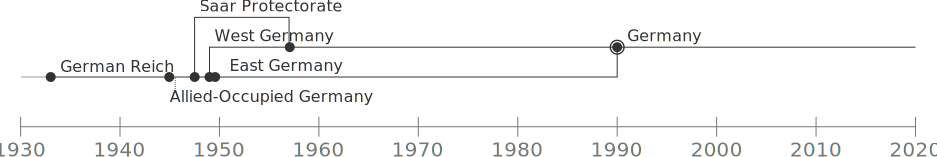
\includegraphics[width=0.8\textwidth]{graphics/development/histograph/example_germany}
  \caption{The concept of the HistoGraph at the example of the history of Germany since 1945}
  \label{fig:example_germany}
\end{figure}

The graph plots Germany first. Since it does not have any successors, the plot goes only one way, historically backwards: East Germany and the Saar Protectorate were incorporated into Germany, so they are plotted. All emerged from the four post-war occupation zones, which are also plotted. All of the four occupation zones themselves originated from the German Reich. However, the German Reich dissolved into many more Areas, e.g. the Memel territory. They are not included in the graph, because they are not predecessors of any Area that is a recursive predecessor of present-day Germany.

Many problems of the graph visualization are apparent in this example: Circles my overlap, if many operations happen in a short period of time -- in this case between 1945 and 1949.
The name ``West Germany'' collides with the vertical line indicating the incorporation of the Saar Protectorate, which should also be avoided.
Additionally, the names of the Areas of the four post-war occupation zones can not be shown in the Graph, because there is no space for them.
One more important aspect can be seen in the creation of West Germany in 1949: A \texttt{UNI} operation unifies three old Areas to one new Area. This could be visualized symmetrically with a straight line from the midmost incoming Area line into the circle to the outgoing Area line of the new Area. This would give the impression that this midmost Area has the same identity than the newly created Area, which is not the case. In general, the circle for \texttt{UNI} and \texttt{SEP} operations with an odd number of old respectively new Areas must be displaced off the center to emphasize that the identity has changed.
All these issues are not in the scope of this thesis and subject to future work in the field of Information Visualization.

% subsection histograph (end)

% ------------------------------------------------------------------------------
\subsection{Edit Mode} % (fold)
\label{sub:edit_mode}

The user interface of HistoGlobe has two modi: The browsing mode to view the evolution of countries on a map with a timeline and the \emph{Edit Mode} to introduce historical changes to Areas. This mode is proposed in this section. The Human Centered Design process produced an interface that allows to intuitively edit Hivents, Areas and historical changes directly in HistoGlobe, without the need to write data into tables or forms. The conceptual model of the interface promotes six Edit Operations, introduced in section \ref{sub:edit_operations}. They describe one historical change that transforms a set of old areas into a set of new areas, using internally the HG Operations (see section \ref{sub:historical_geographic_operations}). In the interface, the historical change is prepared in a workflow of four steps:

\begin{enumerate}
  \item \texttt{SELECT\_OLD\_AREAS}: The user selects the old Areas that will be changed in the Edit Operation.
  \item \texttt{CREATE\_NEW\_TERRITORIES}: For each new Area resulting from the Edit Operation, the user creates a polypolygon describing the territory of the Area.
  \item \texttt{CREATE\_NEW\_NAMES}: Afterwards the user writes the name of each new Area directly on the map. This finalizes the set of new Areas for the historical change.
  \item \texttt{ADD\_CHANGE}: Finally, the historical change has to be added to an Hivent that introduces it and inherits the time point to it. The user either selects an existing Hivent or creates a new one. All the information necessary for the spatio-temporal Hivent Model are completed.
\end{enumerate}

For each Edit Operation, the requirements for the steps are different. Not all operations need all steps and some data is processed automatically. Table \ref{tab:editoperations_in_worklow} presents an overview about the behaviour of each operation in the first three steps. The last step is the same for each operation: Each historical change has to be added to an Hivent.

\begin{table}[H]
\begin{center}
\begin{tabular}{m{0.9cm} m{4.0cm} m{4.4cm} m{3.8cm}}
  \toprule

  &
  \texttt{SELECT\_OLD\_AREAS} &
  \texttt{CREATE\_NEW\_TERRITORIES} &
  \texttt{CREATE\_NEW\_NAMES} \\

  \midrule
  \texttt{CRE} &
  -- &
  \pbox{4.4cm}{create a territory of the new country\\
  \footnotesize{on unclaimed land and/or overlapping existing countries}} &
  create a name of the new country \\

  \midrule
  \texttt{MRG} &
  select the countries to be merged &
  \pbox{4.4cm}{--\\
  \footnotesize{automatic unification of territories of selected countries}} &
  create a name of the merged country
  \\

  \midrule
  \texttt{DIS} &
  select a country to be \mbox{dissolved} &
  create a territory for each new country &
  create a name for each new country \\

  \midrule
  \texttt{CHB} &
  select two neighboring countries to change their border &
  \pbox{4.4cm}{create the new border between both countries \\
  \footnotesize{the territory for both countries will be created automatically}}  &
  -- \\

  \midrule
  \texttt{REN} &
  select a country to change its name &
  -- &
  create a new name of the country \\

  \midrule
  \texttt{CES} &
  select a country to cease it &
  -- &
  -- \\

  \bottomrule
\end{tabular}
\caption{The requirements of each step for the Edit Operations}
\label{tab:editoperations_in_worklow}
\end{center}
\end{table}

% subsection edit_mode (end)

% ------------------------------------------------------------------------------
\subsection{Design Iterations} % (fold)
\label{sub:design_iterations}

The previous sections introduced the concepts of the HistoGraph and the Edit Mode. This section illustrates the Human Centered Design process integrating both concepts into the existing user interface of HistoGlobe. In each phase, interviews with students and employees of Scholar's Lab at University of Virginia were conducted to determine what works well and what has to be improved.

% - - - - - - - - - - - - - - - - - - - - - - - - - - - - - - - - - - - - - - -
\paragraph{Initial interviews} % (fold)
\label{par:initial_interviews}

The first phase, four researchers were asked about their opinions on the idea of HistoGlobe, potential use cases and the concept of the Edit Mode. The idea proved popular, especially for students and teachers in school, historically interested people in general and also for scholars in digital humanities. All researchers agreed that the key to successful Edit Mode is usability, because editing data in time and space is a challenging task. A main concern is uncertainty in historical research: Almost all sorts of information -- temporal, spatial and attribute -- are potentially uncertain. A good user interface for researchers therefore has to support uploading historical sources and indicating uncertainty. The Edit Operations from section \ref{sub:edit_operations} resulted from the initial interviews.

% paragraph initial_interviews (end)


% - - - - - - - - - - - - - - - - - - - - - - - - - - - - - - - - - - - - - - -
\paragraph{Paper Prototype} % (fold)
\label{par:paper_prototype}

From the results of the inital interview, the first interface concept for the Edit Mode was developed and transformed into a paper prototype. It is an interface out of paper that is very fast to create and allows to identify flaws in the concept early in the design process. In this process, two paper prototype iterations were created. Both iteration took about three full work days: one day to create the conceptualize and create prototype, half a day to conduct the study with three people, and one and a half days to analyze the results and rethink the concept.

\begin{figure}[H]
\centering
\begin{subfigure}{.5\textwidth}
  \centering
  \includegraphics[width=225px]{graphics/development/design_process/paper_prototype_1.png}
\end{subfigure}%
\begin{subfigure}{.5\textwidth}
  \centering
  \includegraphics[width=225px]{graphics/development/design_process/paper_prototype_2.png}
\end{subfigure}
\caption{The two iteration of the paper prototype for the Edit Mode}
\label{fig:paper_prototypes}
\end{figure}

The interface consists of a map of Europe, a timeline centered at 1975 and the buttons with a set of dialogs for the for the Edit Mode. Both prototypes were evaluated with three test subjects that had to solve four tasks covering different use cases and operations:
\begin{compactenum}
  \item 1300: Rename incorrectly spelled name of Switzerland on the map (\emph{correction})
  \item 1990: Unite East and West Germany (\emph{forward change})
  \item 1993: Separate the Soviet Union into Russia, Estonia, Latvia, etc. (\emph{forward change})
  \item 1944: Change the border between Finland and the Soviet Union before 1944 (\emph{backward change})
\end{compactenum}

Most parts of the interface concept were understood and all subjects could solve the first three tasks. However, there were also problems:

\begin{compactenum}
  \item There difference between Hivents, the history of a country and an historical change was unclear.
  \item The border drawing dialoge was imagined to be very complex.
  \item The backward change was not understood
  \item Correcting the name Switzerland by changing the event that created it in 1300 caused confusion.
\end{compactenum}

The main finding of this step was that depending on the task, there is both an Hivent-based and an Area-based mental model of the task. This became apparent in the German Reunification Hivent: Some users started the unification operation first, and added West and East Germany afterwards -- and some selected first West Germany, then initiated a unification operation and then added East Germany. From that finding arose that the interface has to support both an Hivent-based and an Area-based approach to introduce historical changes and correct information on the map.

% paragraph paper_prototype (end)

% - - - - - - - - - - - - - - - - - - - - - - - - - - - - - - - - - - - - - - -
\paragraph{Mockup Prototype} % (fold)
\label{par:mockup_prototype}

The main part of the design process was spent on the mockup prototypes. Their purpose is to rapidly develop an interface workflow that is understandable by the users. The prototypes were created in \emph{LibreOffice Impress}, an open-source slide-based presentation tool. The interface is simulated on slides: the map is a background image, the timeline, the set of buttons and dialogs for the Edit Mode and HistoGraph are modelled with geometric elements: lines, circles and rectangles. Interactivity is simulated by linking a click on an element to a different slide that shows the effect of the operation. This allows to model sudden changes in the interface.

\begin{figure}[ht]
  \centering
  \begin{subfigure}[b]{.5\textwidth}
    \centering
    \includegraphics[width=180px]{graphics/development/design_process/mockup_prototype_1.png}
  \end{subfigure}%
  \begin{subfigure}[b]{.5\textwidth}
    \centering
    \includegraphics[width=180px]{graphics/development/design_process/mockup_prototype_3.png}
  \end{subfigure} \\[0.8em]

  % \begin{subfigure}[b]{1.0\textwidth}
  %   \centering
  %   \includegraphics[width=325px]{graphics/development/design_process/mockup_prototype_3.png}
  % \end{subfigure}
  \caption{Two iteration stages of the mockup prototype for the Edit Mode}
  \label{fig:mockup_prototypes}
\end{figure}

Creating the mockup prototype took longer than a paper prototype, but would have still been much faster than actually implementing an interactive Web-based interface. Each prototype iteration was tested with multiple subjects and similar tasks as for the paper prototype. From one test to the next one changes to the interfaces were made. Some interesting quotes from the users were:

\begin{quoteit}
  \begin{tabular}{l r}
    ``this was much easier than I thought'' ~~~~~~~~ &
    ``there is a training session needed'' \\[0.5em]
    ``the interface is very clear &
    ``the logic makes sense, \\
    and graphically pleasing'' &
    it is just very complex'' \\[0.5em]
    ``it's looking good'' &
    ``a nice tutorial and a good \\
    & documentation are necessary'' \\
  \end{tabular}
\end{quoteit}

The main evolution was from a separate dialogue window for the Edit Operation workflow to an intergrated workflow window in the title bar. Also the HistoGraph was introduced to visualize the historical change at while editing it. A lot of smaller design issues, e.g. position of buttons, font sizes or color schemes were identified and fixed. But also conceptual issues arose.

Especially the problem to initiate a backward change (see section \ref{fig:backward_change}) proved to be very difficult. Two design solutions were developed: First, instead of initializing a change in 1990 to separate Germany into East and West, the user can introduce two creation events for the two German states in May and October 1949. The interface needs to provide a visual clue that after creating West Germany, this Area can only be active until 1990, because then another Area, present-day Germany, uses its territory (see figure \ref{sfig:backward_change_1}). The change from West Germany to Germany will be created automatically. The second approach is to introduce a button that flippes an Edit Operation that has just been created (see figure \ref{sfig:backward_change_2}) -- in this case the \texttt{DIS} operation introduced to secede East Germany from Germany will be flipped into a \texttt{UNI} operation to incorporate East Germany into Germany. This approach makes use of the fact that each Edit Operation and has an inverse, as explained in section \ref{par:inverse_operations}.
However, this flipping requires the introduction of additional creation events: West and East Germany were introduced in the change, but only the event that ceases both of them (\texttt{INC} of West Germany into East Germany). They also need a creation event, otherwise they would be active backwards all the way to $t_0$, the initial state of the system.

\begin{figure}[ht]
\centering
\begin{subfigure}[b]{.5\textwidth}
  \centering
  \includegraphics[width=200px]{graphics/development/design_process/backward_change_1.png}
  \caption{Visual clue: predefined and of Area}
  \label{sfig:backward_change_1}
\end{subfigure}%
\begin{subfigure}[b]{.5\textwidth}
  \centering
  \includegraphics[width=200px]{graphics/development/design_process/backward_change_2.png}
  \caption{Create backward change by flipping Edit Operation}
  \label{sfig:backward_change_2}
\end{subfigure}
\caption{Two approaches for editing changes backwards}
\label{fig:backward_change}
\end{figure}

The prototype was very valuable for the development process. In a total of two weeks, an interface concept and workflow was designed that proved to be understandable by the users.


% paragraph mockup_prototype (end)

% - - - - - - - - - - - - - - - - - - - - - - - - - - - - - - - - - - - - - - -
\paragraph{Final Web-based prototype} % (fold)
\label{par:final_web_based_prototype}

The main advantage of the design process is that it prevents major redesigns of the final Web-based prototype. After three months of implementation of the final system, the interface looks very similar to the last version of the mockup prototype. The original main elements of the interface are the map, the timeline with the Now Marker indicating the current date of the visualization and the control buttons for zooming the map and the timeline. They are preserved and extended by new interface elements for the Edit Mode. Their interaction and behavior are introduced in this section at the example of the fictional secession of Scotland from the United Kingdom in 2018. The HistoGraph was not implemented, because of the conceptual problems mentioned in section \ref{sub:histograph} that have to be solved first.

\newpage
\begin{minipage}[t]{0.47\textwidth}

  \begin{figure}[H]
    \centering
    \includegraphics[width=1.0\textwidth]{graphics/development/final_interface/1_init.png}
    \caption{Initial state of the normal mode}
    \label{fig:final_1_init}
  \end{figure}

  The initial state of the user interface. Additional to the original elements, there is an edit button on the upper right corner. Clicking it enters the Edit Mode of the system.

\end{minipage}    % N.B. the % is very important
\hspace{1.5em}    % N.B. this must go in this line, no blank lines !!!
\begin{minipage}[t]{0.47\textwidth}

  \begin{figure}[H]
    \centering
    \includegraphics[width=1.0\textwidth]{graphics/development/final_interface/2_edit_mode.png}
    \caption{Initial state of the Edit Mode}
    \label{fig:final_2_edit_mode}
  \end{figure}

  In the Edit Mode, a title bar and six buttons for the Edit Operations are   revealed. Clicking a button starts the operation workflow introduced in section \ref{par:workflow}.

\end{minipage}

\vspace{1em}
\begin{minipage}[t]{0.47\textwidth}

  \begin{figure}[H]
    \centering
    \includegraphics[width=1.0\textwidth]{graphics/development/final_interface/3_select_old_areas.png}
    \caption{Step 1) \texttt{SELECT\_OLD\_AREAS}}
    \label{fig:final_3_select_old_areas}
  \end{figure}

  A \emph{Workflow Window} is guiding the user through the process of completing the historical change. It shows all the steps necessary for this Edit Operation. In the case of \texttt{DIS}, the user has to select the country to be dissolved by clicking it on the map. After the step is completed, clicking the next button in the workflow window procceeds to the next step. At each point in the workflow, clicking the back button reverts the previous action.

\end{minipage}    % N.B. the % is very important
\hspace{1.5em}    % N.B. this must go in this line, no blank lines !!!
\begin{minipage}[t]{0.47\textwidth}

  \begin{figure}[H]
    \centering
    \includegraphics[width=1.0\textwidth]{graphics/development/final_interface/4_set_new_territories.png}
    \caption{step 2) \texttt{SET\_NEW\_TERRITORIES}}
    \label{fig:final_4_set_new_territories}
  \end{figure}

  In the second step, the user has to create the territory for each new Area that shall be created. Therefore, the \emph{New Territory Tool} provides the functionality to create, manipulate and delete polylines by clicking and moving it directly on the map. The polypolygon drawn by the user is intersected with the old territory to create the territory of the new Area. After one new territory is created sucessfully, the second one can be taken from the remaining old territory by selecting it from the map. As soon as the whole old territory is distributed among the new Areas, the workflow proceeds to the next step.

\end{minipage}

\vspace{1em}
\begin{minipage}[t]{0.47\textwidth}

  \begin{figure}[H]
    \centering
    \includegraphics[width=1.0\textwidth]{graphics/development/final_interface/5_set_new_name.png}
    \caption{Step 3) \texttt{SET\_NEW\_NAMES}}
    \label{fig:final_5_set_new_name}
  \end{figure}

  In the next step, for each Area that has been created in the step before, a name has to be defined. The \emph{New Name Tool} is a draggable input form with two lines, the upper one for the short name, the lower one for the formal name, the identity of the Area. Via instant search, the user can select existing country names from the database to be put in the New Name Tool. When clicking the confirm button, the short name is put directly on the map.

\end{minipage}    % N.B. the % is very important
\hspace{1.5em}    % N.B. this must go in this line, no blank lines !!!
\begin{minipage}[t]{0.47\textwidth}

  \begin{figure}[H]
    \centering
    \includegraphics[width=1.0\textwidth]{graphics/development/final_interface/6_add_change_to_hivent_1.png}
    \caption{Step 4) \texttt{ADD\_CHANGE}}
    \label{fig:final_6_add_change_to_hivent_1}
  \end{figure}

  When all names are set, the Edit Operation is complete. In the last step of the workflow, it has to be added to an Hivent. The \emph{New Hivent Box} offers two possibilities: the user can search for an existing Hivent and add the historical change to it, or create a new one.

\end{minipage}

\vspace{1em}
\begin{minipage}[t]{0.47\textwidth}

  \begin{figure}[H]
    \centering
    \includegraphics[width=1.0\textwidth]{graphics/development/final_interface/7_add_change_to_hivent_2.png}
    \caption{Step 4) \texttt{ADD\_CHANGE}}
    \label{fig:final_7_add_change_to_hivent_2}
  \end{figure}

  The new Hivent created for that change is the ``Scottish Independence'' on 01.01.2018 with a description of the Hivent and possibly a location and a link to a wikipedia article. In the last line, the historical change ``Secession of Scotland from the United Kingdom'' is noted. Clicking the confirm button finalizes the workflow.

\end{minipage}    % N.B. the % is very important
\hspace{1.5em}    % N.B. this must go in this line, no blank lines !!!
\begin{minipage}[t]{0.47\textwidth}

  \begin{figure}[H]
    \centering
    \includegraphics[width=1.0\textwidth]{graphics/development/final_interface/8_final_state.png}
    \caption{The final state with Scotland}
    \label{fig:final_8_final_state}
  \end{figure}

  Clicking the edit button again leaves the Edit mode back to the normal view. Scotland and the United Kingdom are both visible on the map after 2018. When moving the timeline before 2018, Scotland is still part of the UK.

\end{minipage}

% paragraph final_web_based_prototype (end)

% subsection design_iterations (end)

% section user_interface (end)